% Template for PLoS
% Version 3.4 January 2017
%
% % % % % % % % % % % % % % % % % % % % % %
%
% -- IMPORTANT NOTE
%
% This template contains comments intended 
% to minimize problems and delays during our production 
% process. Please follow the template instructions
% whenever possible.
%
% % % % % % % % % % % % % % % % % % % % % % % 
%
% Once your paper is accepted for publication, 
% PLEASE REMOVE ALL TRACKED CHANGES in this file 
% and leave only the final text of your manuscript. 
% PLOS recommends the use of latexdiff to track changes during review, as this will help to maintain a clean tex file.
% Visit https://www.ctan.org/pkg/latexdiff?lang=en for info or contact us at latex@plos.org.
%
%
% There are no restrictions on package use within the LaTeX files except that 
% no packages listed in the template may be deleted.
%
% Please do not include colors or graphics in the text.
%
% The manuscript LaTeX source should be contained within a single file (do not use \input, \externaldocument, or similar commands).
%
% % % % % % % % % % % % % % % % % % % % % % %
%
% -- FIGURES AND TABLES
%
% Please include tables/figure captions directly after the paragraph where they are first cited in the text.
%
% DO NOT INCLUDE GRAPHICS IN YOUR MANUSCRIPT
% - Figures should be uploaded separately from your manuscript file. 
% - Figures generated using LaTeX should be extracted and removed from the PDF before submission. 
% - Figures containing multiple panels/subfigures must be combined into one image file before submission.
% For figure citations, please use "Fig" instead of "Figure".
% See http://journals.plos.org/plosone/s/figures for PLOS figure guidelines.
%
% Tables should be cell-based and may not contain:
% - spacing/line breaks within cells to alter layout or alignment
% - do not nest tabular environments (no tabular environments within tabular environments)
% - no graphics or colored text (cell background color/shading OK)
% See http://journals.plos.org/plosone/s/tables for table guidelines.
%
% For tables that exceed the width of the text column, use the adjustwidth environment as illustrated in the example table in text below.
%
% % % % % % % % % % % % % % % % % % % % % % % %
%
% -- EQUATIONS, MATH SYMBOLS, SUBSCRIPTS, AND SUPERSCRIPTS
%
% IMPORTANT
% Below are a few tips to help format your equations and other special characters according to our specifications. For more tips to help reduce the possibility of formatting errors during conversion, please see our LaTeX guidelines at http://journals.plos.org/plosone/s/latex
%
% For inline equations, please be sure to include all portions of an equation in the math environment.  For example, x$^2$ is incorrect; this should be formatted as $x^2$ (or $\mathrm{x}^2$ if the romanized font is desired).
%
% Do not include text that is not math in the math environment. For example, CO2 should be written as CO\textsubscript{2} instead of CO$_2$.
%
% Please add line breaks to long display equations when possible in order to fit size of the column. 
%
% For inline equations, please do not include punctuation (commas, etc) within the math environment unless this is part of the equation.
%
% When adding superscript or subscripts outside of brackets/braces, please group using {}.  For example, change "[U(D,E,\gamma)]^2" to "{[U(D,E,\gamma)]}^2". 
%
% Do not use \cal for caligraphic font.  Instead, use \mathcal{}
%
% % % % % % % % % % % % % % % % % % % % % % % % 
%
% Please contact latex@plos.org with any questions.
%
% % % % % % % % % % % % % % % % % % % % % % % %

\documentclass[10pt,letterpaper]{article}
\usepackage[top=0.85in,left=2.75in,footskip=0.75in]{geometry}

% amsmath and amssymb packages, useful for mathematical formulas and symbols
\usepackage{amsmath,amssymb}

% Use adjustwidth environment to exceed column width (see example table in text)
\usepackage{changepage}

% Use Unicode characters when possible
\usepackage[utf8x]{inputenc}

% textcomp package and marvosym package for additional characters
\usepackage{textcomp,marvosym}

% cite package, to clean up citations in the main text. Do not remove.
\usepackage{cite}

% Use nameref to cite supporting information files (see Supporting Information section for more info)
\usepackage{nameref,hyperref}

% line numbers
\usepackage[right]{lineno}

% ligatures disabled
\usepackage{microtype}
\DisableLigatures[f]{encoding = *, family = * }

% color can be used to apply background shading to table cells only
\usepackage[table]{xcolor}

% array package and thick rules for tables
\usepackage{array}

\usepackage{afterpage}
\usepackage{caption, subcaption, multirow, morefloats}

% create "+" rule type for thick vertical lines
\newcolumntype{+}{!{\vrule width 2pt}}

% create \thickcline for thick horizontal lines of variable length
\newlength\savedwidth
\newcommand\thickcline[1]{%
  \noalign{\global\savedwidth\arrayrulewidth\global\arrayrulewidth 2pt}%
  \cline{#1}%
  \noalign{\vskip\arrayrulewidth}%
  \noalign{\global\arrayrulewidth\savedwidth}%
}

% \thickhline command for thick horizontal lines that span the table
\newcommand\thickhline{\noalign{\global\savedwidth\arrayrulewidth\global\arrayrulewidth 2pt}%
\hline
\noalign{\global\arrayrulewidth\savedwidth}}


% Remove comment for double spacing
%\usepackage{setspace} 
%\doublespacing

% Text layout
\raggedright
\setlength{\parindent}{0.5cm}
\textwidth 5.25in 
\textheight 8.75in

% Bold the 'Figure #' in the caption and separate it from the title/caption with a period
% Captions will be left justified
\usepackage[aboveskip=1pt,labelfont=bf,labelsep=period,justification=raggedright,singlelinecheck=off]{caption}
\renewcommand{\figurename}{Fig}

% Use the PLoS provided BiBTeX style
\bibliographystyle{plos2015}

% Remove brackets from numbering in List of References
\makeatletter
\renewcommand{\@biblabel}[1]{\quad#1.}
\makeatother

% Leave date blank
\date{}

% Header and Footer with logo
\usepackage{lastpage,fancyhdr,graphicx}
\usepackage{epstopdf}
\pagestyle{myheadings}
\pagestyle{fancy}
\fancyhf{}
\setlength{\headheight}{27.023pt}
\lhead{\includegraphics[width=2.0in]{PLOS-submission.eps}}
\rfoot{\thepage/\pageref{LastPage}}
\renewcommand{\footrule}{\hrule height 2pt \vspace{2mm}}
\fancyheadoffset[L]{2.25in}
\fancyfootoffset[L]{2.25in}
\lfoot{\sf PLOS}

%% Include all macros below

\newcommand{\lorem}{{\bf LOREM}}
\newcommand{\ipsum}{{\bf IPSUM}}

%% END MACROS SECTION


\begin{document}
\vspace*{0.2in}

% Title must be 250 characters or less.
\begin{flushleft}
  {\Large
  \textbf\newline{Ensemble approaches for estimating congruence between species delimitation and morphological variation: a case study using the Pacific Pond Turtle (\textit{Emys marmorata})} % Please use "sentence case" for title and headings (capitalize only the first word in a title (or heading), the first word in a subtitle (or subheading), and any proper nouns).
  }
  \newline
  % Insert author names, affiliations and corresponding author email (do not include titles, positions, or degrees).
  \\
  Peter D Smits\textsuperscript{1*},
  Kenneth D Angielczyk\textsuperscript{2},
  Bryan L Stuart\textsuperscript{3},
  James F Parham\textsuperscript{4},
  \\
  \bigskip
  \textbf{1} Department of Integrative Biology, University of California -- Berkeley, Berkeley, California, USA.
  \\
  \textbf{2} Integrative Research Center, Field Museum of Natural History, Chicago, Illinois, USA.
  \\
  \textbf{3} Section of Research and Collections, North Carolina Museum of Natural Sciences, Raleigh, North Carolina, USA.
  \\
  \textbf{4} Department of Geological Sciences, California State University -- Fullerton, Fullerton, California, USA.
  \\
  \bigskip

  % Insert additional author notes using the symbols described below. Insert symbol callouts after author names as necessary.
  % 
  % Remove or comment out the author notes below if they aren't used.
  %
  % Primary Equal Contribution Note
  %\Yinyang These authors contributed equally to this work.

  % Additional Equal Contribution Note
  % Also use this double-dagger symbol for special authorship notes, such as senior authorship.
  %\ddag These authors also contributed equally to this work.

  % Current address notes
  %\textcurrency Current Address: Dept/Program/Center, Institution Name, City, State, Country % change symbol to "\textcurrency a" if more than one current address note
  % \textcurrency b Insert second current address 
  % \textcurrency c Insert third current address

  % Deceased author note
  %\dag Deceased

  % Group/Consortium Author Note
  %\textpilcrow Membership list can be found in the Acknowledgments section.

  % Use the asterisk to denote corresponding authorship and provide email address in note below.
  * psmits@berkeley.edu

\end{flushleft}
% Please keep the abstract below 300 words
\section*{Abstract}
  We investigated the morphometric identification of cryptic species using machine learning approaches by examining their implications for a recently proposed cryptic turtle species (\textit{Emys pallida}). We used landmark-based morphometric data to quantify plastron shape in 532 adult \textit{E. marmorata/``E. pallida''} museum specimens. We assigned a classification to each specimen for six different binning schemes based on geographic occurrence data recorded in museum collection archives. We used an ensemble of supervised machine learning approaches to determine which classification hypothesis was best supported by the data. In addition, we applied the same approach to two clear-cut examples, one consisting of seven unambiguously distinct species closely related to \textit{E. marmorata} and an outgroup (\textit{Chrysemys picta}), and the other consisting of two subspecies of \textit{Trachemys scripta}. The analyses of the clear-cut examples produced near perfect classifications, demonstrating that plastron shape typically is a useful marker for differentiating turtle species, and that the methods can recover correct results when an appropriate signa exists. There is no clear ``best'' grouping of \textit{E. marmorata/``E. pallida''} based on plastron shape. Explanations for the lack of grouping in \textit{E. marmorata} include the possibility that genetic differentiation is not associated with plastron shape variation below the species level and/or that local selective pressures (e.g., from hydrological regime) overwhelm morphological differentiation. A reconsideration of the methods used to delimit \textit{``E. pallida,''} the lack of barriers to gene flow, the strong evidence for widespread admixture between lineages, and the fact that plastron shape can be used to delineate other emydid species and sub-species suggest that its lack of diagnosability most likely reflects the non-distinctiveness of this proposed taxon. 


  % Please keep the Author Summary between 150 and 200 words
  % Use first person. PLOS ONE authors please skip this step. 
  % Author Summary not valid for PLOS ONE submissions.   
  %\section*{Author summary}

\linenumbers

% Use "Eq" instead of "Equation" for equation citations.
\section*{Introduction}

% cryptic diversity
%   most species are still deliminated solely based on morphology
Molecular systematics has repeatedly demonstrated the existence of cryptic species that can only be diagnosed using genetic data \cite{Stuart2006,Bickford2007,SchlickSteiner2007,Pfenninger2007,Clare2011,Funk2012}. In attempts to streamline the documentation of biodiversity, several methods of species delimitation that rely almost entirely on genetic data have recently been proposed \cite{Pons2006,Carstens2010,Hausdorf2010,O'Meara2010,Yang2010b,Huelsenbeck2011b}. Although strong caveats on the utility of these methods have been raised \cite{Bauer2000,Carstens2013}, they are nevertheless being used to name species \cite{Leache2010,Spinks2014}.

In contrast to those genetically-diagnosed species, the majority of extant taxa, and almost all extinct taxa, are delimited by morphology alone. This disjunction complicates interpretations of variation and diversity in deep time, as apparent morphological stasis may not reflect the true underlying diversity \cite{Eldredge1972,Gould1977a,VanBocxlaer2013}. It also has serious implications for our records of modern biodiversity: for many museum specimens of extant taxa (e.g. those preserved in formalin), it is difficult to acquire the genetic data needed for non-morphological species delimitation methods.

These considerations have sparked interest in whether geometric morphometric analyses can capture fine-scale variation that can be used for identifying cryptic species. Most studies focus on using morphometrics to discover differences between taxa that were identified by other means \cite{Polly2003,Zelditch2004,Gaubert2005b,Gunduz2007,Polly2007a,Demandt2009,Markolf2013,Fruciano2016}. Additionally, there has been work on automated taxon identification and classification of taxa into groups \cite{Baylac2003,Dobigny2003,MacLeod2007,VandenBrink2011,Vitek2017}, as well as the development of models that combine genetic, phenotypic, and geographic data to infer evolutionary units of interest \cite{Guillot2012}.

Here, we investigate the morphometric identification of cryptic species using machine learning approaches. We use an ensemble learning approach where multiple methods are used in order to look for consensus among their results. We test our approach on three datasets: plastron (ventral shell) shape of seven species of closely related turtles and one outgroup, plastron shape of two subspecies of a single turtle species, and plastron shape of the \textit{Emys marmorata} species complex. In particular, we ask whether it is possible to determine which among a set of classification hypotheses best aligns with the observed morphology, and examine the implications of our results for the \textit{E. marmorata} complex. 

% past work on automatic taxon identification and older approaches to classifying taxa
% why use machine learning methods
\subsection*{Background and study system}
Machine learning is an extension of known statistical methodology that emphasizes predictive accuracy and generality, often at the expense of the interpretability of individual parameters \cite{Hastie2009}. Basic statistical approaches are supplemented by randomization, sorting, and partitioning algorithms, along with the maximization or minimization of summary statistics, in order to best estimate a general model for all data, both sampled and unsampled \cite{Hastie2009}. Machine learning approaches have found use in medical research, epidemiology, economics, and automated identification of images such as handwritten zip codes \cite{Hastie2009}. % additional/more specific CITATIONS?

There are two major classes of machine learning methods: unsupervised and supervised learning. Unsupervised learning methods are used with unlabeled data where the underlying structure is estimated; they are analogous to clustering and density estimation methods \cite{Kaufman1990}. Supervised learning methods are used with labeled data where the final output of data is known and the rules for going from input to output are inferred. These are analogous to classification and regression models \cite{Breiman1984,Hastie2009}. Our application of the supervised learning approaches used in this study illustrates only a sampling of the various methods available for fitting classification models. The specific methods we used were chosen because they are suited for cases with more two or more response classes.

Geometric morphometric approaches to identifying differences in morphological variation between classes, including cryptic species, have mostly relied on methods like linear discriminate analysis and canonical variates analysis \cite{Polly2003,Zelditch2004,Gaubert2005b,Gunduz2007,Polly2007a,Francoy2009,Sztencel-Jabonka2009,Edwards2011,MitrovskiBogdanovic2013,Dillard2017}. Because of their similarity to multivariate approaches like principal components analysis (PCA), these methods are comparatively straightforward ways of understanding the differences in morphology between classes. They also benefit from producing results that can be easily visualized, which aids in the interpretation and presentation of data and results. Most previous morphometric studies did not assess which amongst a set of alternative classification hypotheses was optimal. For example, studies such as those of Camul et al. \cite{Caumul2005a} and Polly \cite{Polly2007a} focused on comparing different aspects of morphology and their fidelity to a classification scheme instead of comparing the fidelity of one aspect of morphology to multiple classification schemes. In this context, the study of Cardini et al. \cite{Cardini2009a} is noteworthy because they compared morphological variation in marmots at the population, regional, and species level and determined the fidelity of shape to divisions at each of these levels.

Here, we used an ensemble of supervised machine learning methods to compare the congruence of morphological data to different classification hypotheses. Each of these methods provide different advantages for understanding how to classify specimens, as well as the accuracy of the resulting classifications. 
Machine learning methods have been combined with geometric morphometric data to study shape variation in a variety of contexts, including automated taxon identification and classification of groups \cite{Baylac2003,Dobigny2003,MacLeod2007,VanBocxlaer2010,VandenBrink2011,Navega2015}. % MORE
%Although machine learning methods such as neural networks have been applied to studying shape variation, including in the context of automated taxon identification and classification of groups, the number of cases remains limited. 
In the current study, we not only consider pure classification accuracy but also use a statistic of classification strength that reflects the rate at which taxa are both accurately and inaccurately classified: the area under the Receiver Operating Characteristic curve \cite{Hastie2009}. 

We analyzed the problem of whether there are distinct subspecies or cryptic species within the western pond turtle, \textit{Emys marmorata} \cite{Baird1852} (formerly \emph{Clemmys marmorata}; see \cite{Feldman2002}). \textit{Emys marmorata} is distributed from northern Washington State, USA to Baja California, Mexico; populations in western Nevada may have been introduced by recent human activity or they could be a genuine part of the species' range \cite{Bury2017}. Traditionally, \textit{E. marmorata} was classified into two named subspecies: the northern \textit{E. marmorata marmorata} and the southern \textit{Emys marmorata pallida} \cite{Seeliger1945}, with a central Californian intergrade zone in between. \textit{Emys marmorata marmorata} is differentiated from \textit{E. marmorata pallida} by the presence of a pair of triangular inguinal scales and darker neck markings. The triangular inguinal plates can sometimes be present in \textit{E. marmorata pallida} although they are considerably smaller. Seeliger \cite{Seeliger1945} did not formally include the Baja California populations of \textit{E. marmorata} in either taxon, implying the existence of a third distinct but unnamed subspecies.

Previous work on morphological variation in \textit{E. marmorata} has focused primarily on differentiation between populations over a portion of the species' total range \cite{Lubcke2007,Germano2008,Germano2009,Bury2010}; comparatively few studies have included specimens from across the entire range \cite{Holland1992}. Most of these studies considered how local biotic and abiotic factors may contribute to differences in carapace length, and they found that size can vary greatly between different populations \cite{Lubcke2007,Germano2008,Germano2009}. There also has been interest in size-based sexual dimorphism in \textit{E. marmorata} \cite{Holland1992,Lubcke2007,Germano2009}, with males being on average larger than females based on total carapace length and other linear measurements. However, the quality of size as a classifier of sex can vary greatly between populations \cite{Holland1992} because of the magnitude of size differences among populations \cite{Lubcke2007,Germano2009}. The effect of sexual dimorphism on shape, \textit{sensu} Kendall \cite{Kendall1977a}, has not been assessed \cite{Holland1992,Lubcke2007,Germano2008}.

Of particular relevance in the context of cryptic diversity in \textit{E. marmorata} is the morphometric analysis of carapace shape carried out by Holland \cite{Holland1992}, who compared populations of \textit{E. marmorata} from three areas of the species' range. Holland concluded that geographic distance was a poor indicator of morphological differentiation, and instead hypothesized that geographic features such as breaks between different drainage basis are probably more important barriers to dispersal and interbreeding. Additionally, he suggested that morphological differences were more pronounced as the magnitude of barriers and distance increased, but this variation required many variables to adequately capture, implying only very subtle morphological differentiation between putatively distinct populations. Finally, Holland concluded that \textit{E. marmorata} is best classified as three distinct species: a northern species, a southern species, and a Columbia Basin species. This classification is similar to that of \cite{Seeliger1945}, except elevated to the species level and without recognition of a distinct Baja species. 

More recently, the phylogeography of \textit{E. marmorata} and the possibility of cryptic diversity was investigated using molecular data \cite{Spinks2005,Spinks2010,Spinks2014}. Based on mitochondrial DNA, Spinks and Shaffer \cite{Spinks2005} recognized four subclades within \textit{E. marmorata}, a northern clade, a San Joaquin Valley clade, a Santa Barbara clade, and a southern clade. Analyses with nuclear DNA \cite{Spinks2010} and single-nucleotide polymorphism (SNP) data suggest a primarily north--south division in \textit{E. marmorata}, although these datasets differed from the mitocondrial-based results of Spinks and Shaffer \cite{Spinks2005} in the location of the break point \cite{Spinks2014}. All three studies discussed the potential taxonomic implications of their results, with Spinks et al. \cite{Spinks2014} going so far as to strongly advocate for the recognition of at least two species (\emph{E. marmorata} and \emph{E. pallida}), and a possible third based on populations in Baja California. However, they did not discuss in detail the morphological characters that would help to diagnose these species beyond those specified by Seeliger \cite{Seeliger1945}. Given that these characters are variable within the proposed species, and that Holland \cite{Holland1992} described shell shape variation that might be consistent with this taxonomy, a geometric morphometric analysis of shell shape might provide a reliable way to diagnose groups (whether species or subspecies) within \textit{E. marmorata}.

In this study, we attempt to estimate the best classification scheme of \textit{E. marmorata} based on variation in plastron (ventral shell) shape in order to determine whether this character is consistent with any of the proposed taxonomies of the \textit{E. marmorata} complex. 

We choose to analyze plastron shape for multiple reasons. First, it is very easy to collect geometric morphometric data on plastron shape from two-dimensional photographs as the structure is virtually flat. This approach allows both museum specimens and individuals photographed in the field to be analyzed together. Second, previous work has suggested that there are strong differences in plastron shape among traditionally-recognized emydine species \cite{Angielczyk2007,Angielczyk2011,Angielczyk2013a}. Finally, due to these previous studies a large dataset was readily available.

In the case of the \textit{E. marmorata} species complex, we hypothesize that if one or more of the proposed classification schemes are consistent with the morphological data then our ensemble approach fit to those hypotheses will have higher out-of-sample predictive performance than the more inconsistent hypotheses. However, if all of the classification schemes lead to equal out-of-sample predictive performance then we would conclude that the proposed hypotheses are inconsistent with whatever information is present in the morphological data. Because of unclear geographic boundaries between subgroups of \textit{E. marmorata}, we compare multiple permutations of the Spinks et al. \cite{Spinks2010} and Spinks et al. \cite{Spinks2014} hypotheses.





\section*{Materials and methods}
\subsection*{Specimens, sampling, morphometrics}


Three different geometric morphometric datasets describing turtle plastron variation were assembled for this analysis: 1) specimens from seven distinct emydine species and a deriochelyine outgroup (\textit{C. picta}); 2) \textit{T. scripta} specimens from the two main subspecies (\textit{T. scripta elegans} and \textit{T. scripta scripta}); and 3) \textit{E. marmorata} specimens from across the species' geographic range. The first two datasets are intended to serve as a test of whether machine learning techniques can differentiate species-level groupings of emydid turtles using plastron shape. We expect that the first case represents a low complexity dataset because of the high level of plastron shape disparity that exists among these species \cite{Claude2003a,Claude2006,Angielczyk2011}, whereas the second dataset should be relatively higher in complexity and more analogous to the \textit{E. marmorata} example. We predict that the \textit{E. marmorata} dataset should be of the highest complexity and our greatest challenge given the previous finding that only very subtle differences existed between geographically-distinct populations \cite{Holland1992}.

The first dataset we analyzed includes 578 total specimens from the following species: \textit{Chrysemys picta}, \textit{Clemmys guttata}, \textit{Emys blandigii}, \textit{Emys orbicularis}, \textit{Glyptemys insculpta}, \textit{Glyptemys muhlenbergii}, \textit{Terrapene coahuila}, and \textit{Terrapene ornata}. These specimens are a subset of those used in previous studies \cite{Angielczyk2011,Angielczyk2013a}.

The second dataset is a compilation of 101 specimens of two subspecies of \textit{T. scripta}: 51 specimens of \textit{T. scripta scripta} and 50 specimens of \textit{T. scripta elegans}. These landmark data are new to this study. 

The final dataset is of 532 adult \textit{E. marmorata} museum specimens, though not all specimens were able to be assigned a class for all schemes (Fig. \ref{fig:map}). These specimens represent a subset of those included in previous studies \cite{Angielczyk2007,Angielczyk2011,Angielczyk2013a}. Because previous genetic studies did not use vouchered specimens \cite{Spinks2005,Spinks2010,Spinks2014} we were not able to directly sample the individuals in their studies. Instead, our specimen classifications were based solely on the geographic information and not explicit assignment using molecular data. For each taxonomic hypothesis, specimens were assigned to one of the possible classes based on geographic occurrence data recorded in museum collections. In cases where precise latitude and longitude information were not available we estimated them from other locality information. Because the exact barriers between different biogeographic regions are unknown and unclear, we represented each hypothesis with multiple possible realizations representing the classification uncertainty for specimens present at the geographic boundaries. The taxonomic hypotheses and sub-hypotheses for \textit{E. marmorata} used here are presented in Table \ref{tab:hypotheses} and Fig. \ref{fig:map}.

\begin{table}
  \centering
    \caption{Table of species delimitation hypotheses for \textit{E. marmorata}}
    \begin{tabular}{l l l }
      \hline
      Abbreviation & Number of classes & citation \\
      \hline
      SP10.1 & 3 & \cite{Spinks2010} \\
      SP10.2 & 3 & \cite{Spinks2010} \\
      SP10.3 & 4 & \cite{Spinks2010} \\
      SP14.1 & 2 & \cite{Spinks2014} \\
      SP14.2 & 4 & \cite{Spinks2014} \\
      Morph & 2 & \cite{Spinks2010} \\
      \hline
    \end{tabular}
    \label{tab:hypotheses}
\end{table}

\afterpage{\clearpage}
\begin{figure}[ht]
  \centering
  %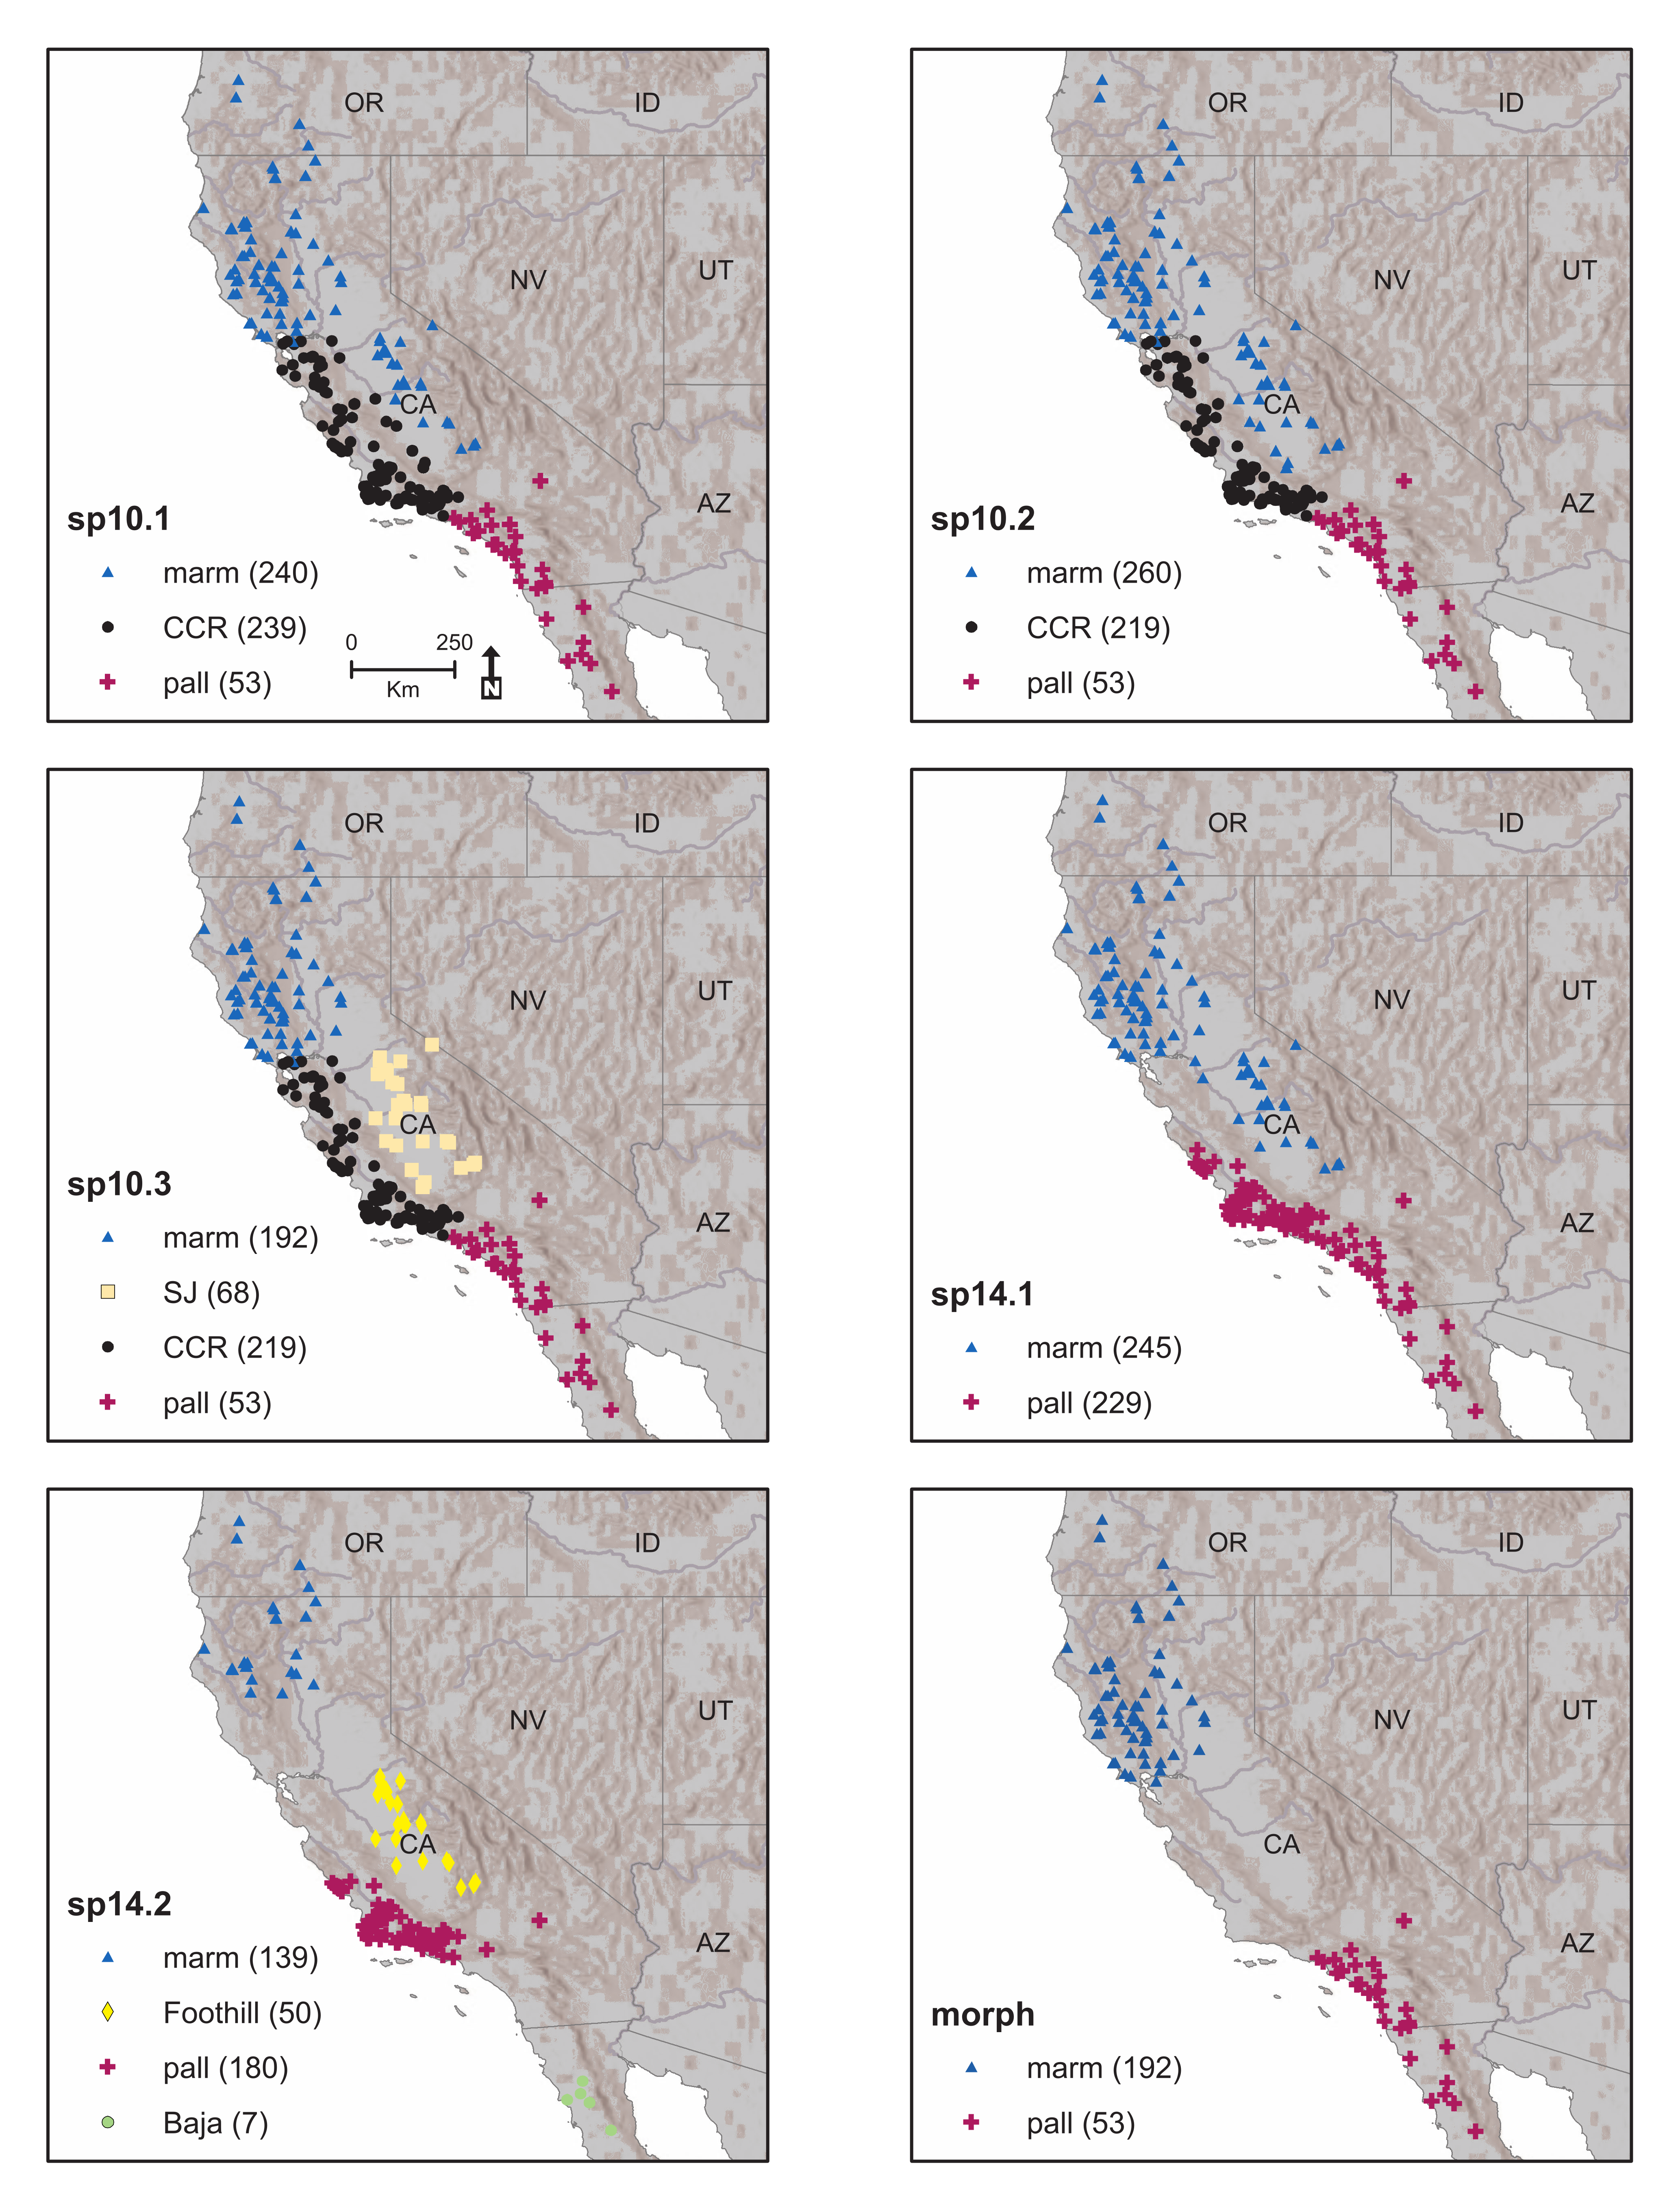
\includegraphics[height = 0.8\textheight, width = \textwidth, keepaspectratio = true]{figure/Ken_Ang_SpLoc_final_comp}
  \caption{Geographic distribution of specimens sampled for comparing the hypothesized subdivisions of \textit{Emys marmorata}. Each hypothesized scheme has two or more possible classes. Sample size differs between schemes because of our ability to confidently assign museum specimens to the various schemes. The number of localities shown on each map is less than the number of specimens sampled because some localities produced multiple specimens. The different classification abbreviations are as follows: \textit{E. marmorata} = ``marm'', \textit{E. pallida} = ``pall'', Central Coast Ranges = ``CCR'', San Joaquin Valley = ``SJ,'' Baya Peninsula = ``Baja,'', and Sierra Foothills = ``Foothill.''}
  \label{fig:map}
\end{figure}


We used three main binning schemes. All three schemes include a class for \textit{E. marmorata} specimens from northern populations (marm) as well as a class for those assigned to \textit{E. pallida} (pall) and an intergrade zone in the Central Coast Ranges (CCR). The schemes differ in the assignment of samples from the San Joaquin Valley (Fig. \ref{fig:map}). Scheme SP10.1 and SP10.2 differ in the assignment of specimens from the western San Joaquin Valley to either CCR or marm reflecting uncertainty regarding their genetic affinity as explained above. In scheme SP10.3 these specimens are assigned to a San Joaquin class reflecting the mitochondrial distinctiveness shown by Spinks and Shaffer \cite{Spinks2005}. We used two versions of the binning scheme based on the results of Spinks et al. \cite{Spinks2014}: SP14.1 reflects their phylogenetic network analysis and SP14.2 corresponds to their Bayesian species delimitation analysis. SP14.2 requires the addition of two new classes, ``Baja'' and ``Foothill,'' to accommodate the genetic groupings recovered by the SNP Structure analysis that was used to create the guide tree for the BPP species delimitation analysis \cite{Spinks2014}. Finally, we proposed a conservative morphological scheme (``Morph'') in order to compare the molecular hypotheses with something approximating the original taxonomic hypothesis for the group. This scheme is made up solely of the marm and pall classes from the SP10.3 scheme.


Sex was known only for a subset of the total dataset and was not included as a predictor of classification. Instead, we estimated the degree to which specimens cluster morphologically by sex in order to determine how much of a potential biasing factor sexual dimorphism could be for our analysis of the \textit{E. marmorata} species complex (see below).

Following previous work on plastron shape \cite{Angielczyk2007,Angielczyk2011,Angielczyk2013a}, we used TpsDig 2.04 \cite{Rohlf2005} to digitize 19 two-dimensional landmarks (Fig. \ref{fig:plastra}). Seventeen of the landmarks are at the endpoints or intersection of the keratinous scutes that cover the plastron. Twelve of the landmarks were symmetrical across the axis of symmetry. Because damage prevented the digitization of all the symmetric landmarks in some specimens, we reflected landmarks across the axis of symmetry (i.e. midline) prior to analysis and used the average position of each symmetric pair. In cases where damage or incompleteness prevented symmetric landmarks from being determined, we used only the single member of the pair. We conducted all subsequent analyses on the resulting ``half'' plastra. We superimposed the plastral landmark configurations using generalized Procrustes analysis \cite{Dryden1998a}, after which we calculated the principal components (PC) of shape using the \texttt{shapes} package for R \cite{R2016,Dryden2013}. All specimens were used for superimposition, after which the subset labeled for each of the schemes were used in model training and testing (see below).

\begin{figure}[ht]
  \centering
  %\includegraphics[height = 0.5\textheight, width = \textwidth, keepaspectratio = true]{figure/plastra}
  \caption{Depiction of general plastral shape of \textit{E. marmorata} and position of the 19 landmarks used in this study. Anterior is towards the top of the figure.}
  \label{fig:plastra}
\end{figure}

\subsection*{Biasing effects}
% digitization
We estimated the possible effect of digitization error \cite{Arnqvist1998,Cramon2007,Munoz-MunozF.2010} on our results by comparing within-specimen (replicated) Procrustes distances to the distances between classification scheme centroids. Ten randomly-selected \textit{E. marmorata} specimens were each digitized four times, with the original set of digitized coordinates serving as a fifth replicate. These 50 landmark configurations were Procrustes superimposed. A range of four Procrustes distances was then calculated as the average of the pairwise distances between each of the replicate configurations of a given specimen.

For each specimen, the difference in shape caused by digitization was calculated as the mean of all pairwise Procrustes distances between the five replicates of that specimen. The average distance between any two digitizations was calculated as the mean of all pairwise Procrustes distances between all replicates for all specimens. The ratio between these two values was used to assess the magnitude of variation caused by digitization. The goal of this ratio is to determine if the within group distances are smaller on average than the between individual distances; a value of 0 indicates perfect grouping, a value of 1 indicates no difference between grouping and no grouping, and a value of 1+ indicates that the grouping is counter-intuitive to the data.

\textit{Emys marmorata} is known to display sexual dimorphism in plastral shape, particularly the presence of a plastral concavity in males \cite{Seeliger1945}. To test for biases resulting from sexual dimorphism in our \textit{E. marmorata} dataset, we used a simple permutation test to determine if the distance between the mean female and male shapes is greater than expected when the sex labels are randomly shuffled. Because not all of our specimens have sex identifications associated with them, this analysis was done using a subset of the data (257 of 532). This analysis was also done for each of the classification schemes in order to determine if sex is a biasing factor within these groups. As with the total dataset, only a limited number of specimens in each classification scheme have sex information, and the observed sex ratios for each of the classes within the classification schemes are summarized in Table \ref{tab:sex_ratio}. Importantly, these within-class sex ratios are based only on the subset of specimens with sex information.

\begin{table}
  \centering
  \caption{Table of within-class sex ratios from those speciems with sex information for ecah classification schemes used in this analysis.}
    \begin{tabular}{l l}
      \hline
      Scheme & class ratios \\
      \hline
      SP10.1 & CCR: 70 F/60 M; Marm: 112/113; Pall: 20/26 \\
      SP10.2 &  CCR: 63/50; Marm: 119/123; Pall: 20/26 \\
      SP10.3 & CCR: 63/50; Marm: 92/95; Pall: 20/26; SJ: 27/28 \\
      SP14.1 & Marm: 112/117; Pall: 65/61 \\
      SP14.2 & Baja: 0/5; Foothill: 20/19; Marm: 70/63; Pall: 45/38\\
      Morph & Marm: 92/94; Pall: 20/26 \\
      \hline
    \end{tabular}
  \label{tab:sex_ratio}
\end{table}



\subsection*{Supervised learning approaches}

Instead of relying on a single supervised learning method, we chose to use an ensemble approach where multiple model types are used in concert so that any congruence between them increases our support for that conclusion over another \cite{Hastie2009}. The supervised learning methods used here are named in Table \ref{tab:methods}. Each of these methods makes different assumptions, treats data differently, and can produce different classification results depending on the nature of the data \cite{Hastie2009}. For example, multinomial logistic regression is a type of generalized linear model, whereas random forest is itself an ensemble approach where multiple decision trees are fit to subsets of the full dataset and then averaged.

\begin{table}
  \centering
  \caption{Table of the supervised learning methods used in this analysis.}
  \scalebox{0.9}{
    \begin{tabular}{l l l l}
      \hline
      Method name & abbreviation & R package & citation \\
      \hline
      multinomial logistic regression & MLR & nnet & \cite{Venables2002} \\
      linear discriminate analysis & LDA & MASS & \cite{Venables2002} \\
      penalized discrminiate analysis & PDA & mda & \cite{mdapack} \\
      single-hidden-layer neural network & NN & nnet & \cite{Venables2002} \\
      random forests & RF & randomForest & \cite{Liaw2002} \\
      \hline
    \end{tabular}}
  \label{tab:methods}
\end{table}

The maximum set of possible predictors or features used for any model of our dataset is comprised of the first 25 principal components (PCs), scaled centroid size, the interaction between scaled centroid size and PC 1, and the interaction between scaled centroid size and PC 2. Additional interaction terms were not considered because of model complexity/sample size concerns. Size and the interaction between size and PCs 1 and 2 were included as predictors to account for known ontogenetic variation in plastron shape \cite{Angielczyk2013a} as well as potential size differences between classes, even if this is unlikely \cite{Seeliger1945,Holland1992}. These data constitute a ``maximum set'' because the best or selected models based on five-fold cross-validation need not, and likely will not, include all predictors possible (see below). Because our supervised learning models use PCs as predictors, this approach is in many ways analogous to PCA regression. PCA regression takes advantage of the reduction and orthogonality PCs to improve regression fit \cite{Hastie2009}. Because the PCs of shape are by definition orthogonal, they can easily serve as independent predictors or features of class membership without fear of collinearity.


We adopted a training and testing paradigm for selecting parsimonious models and estimating their overall error rates \cite{Hastie2009,Kuhn2013}. Within-sample model performance is inherently biased upwards, so model evaluation requires overcoming this bias. With very large sample sizes, as in this study, part of the sample can be used as the ``training set'' and the remainder acts as the ``testing set.'' In this approach, following all cleaning and vetting, the data are split into a training dataset and a testing dataset. The former is used for fitting the model whereas the later is used for measuring model performance, a process called model generalization. For each scheme, we limited the model training and testing to only those individuals with class labels for that scheme. In this analysis, we randomly divided 80\% of samples into the training set and the remaining 20\% into the testing set. 

In classification studies, such as this one, a common metric of performance is the receiver operating characteristic (ROC) which is the relationship between the false and true positive rates \cite{Hastie2009}. The area under the ROC curve (AUC) is the derived estimate of model performance; AUC ranges from 0.5 to 1 which correspond to performance similar to random guesses and perfect classification rates, respectively \cite{Hastie2009}. Both ROC and AUC are preferable to simple classification accuracy when class membership is unbalanced, as it is in these analyses \cite{Hastie2009}. The standard ROC and AUC calculations are defined only for binary classifications, which is not the case for our eight species and \textit{Emys} complex datasets. To generalize this approach for situations with multiple response classes, we used an all-against-one strategy where the model AUC is the average of the AUC values from the multiple binary comparisons of one class compared to all others \cite{Hand2001}. 

For a given supervised learning method, we compared the fit of 27 models as the average AUC from 10 rounds of five-fold cross-validation. Cross-validation is an approach for estimating the average out-of-sample predictive error of a model by simulating out-of-sample data from the training dataset itself \cite{Hastie2009}. In a single round of \(k\)-fold cross-validation, the training data are divided into \(k\) blocks where the model is fit to \(k - 1\) blocks and the values of the \(k\)th block are predicted. This is repeated for all combinations of blocks. Within each round, the predictive performance metrics are averaged across all folds. Finally, the predictive performance metric is the averaged across all rounds of \(k\)-fold cross-validation. This process was implemented using the R package \texttt{caret} \cite{KuhnMAN2013}. For a given supervised learning method, the ``best'' trained model is that with the highest mean AUC as estimated from five-fold cross-validation. The selected or final model, however, is the next most parsimonious model that is within one standard error of the best model; this is a variant on the ``one-standard error'' rule \cite{Hastie2009}. The purpose of this rule is to ameliorate the chances of selecting an overly complex model that will perform poorly when predicting the classes of out-of-sample data.



\section*{Results}

\subsection*{Geometric morphometrics}

The results of the PCA of plastron shape in both the eight species and \textit{Trachemys} datasets demonstrate strong association between shape and the recognized classification schemes (Fig. \ref{fig:other_pca}).

\begin{figure}[h]
  \centering
  %\includegraphics[height = \textheight, width = \textwidth, keepaspectratio = true]{figure/other_pc_graph}
  \caption{Two scatterplots of morphological differences from two of the three datasets analyzed in this study. (a) Scatterplot of the first two PCA axies from the landmarks from the eight different species dataset, and (b) the first two axes of variation from two subspecies of \textit{Trachemys} dataset. Point colors correspond to the categories within each dataset while point size is proportional to individual centroid size. In parentheses next to the axis labels are the percent of total variation accounted for by that axis. For both datasets there are clear distinctions between the different categories.}
  \label{fig:other_pca}
\end{figure}

The results of the PCA of plastron shape in the \textit{Emys marmorata} dataset show no clear connection between plastron shape and any of the proposed classification schemes (Fig. \ref{fig:emys_pca}). The first PC axis of shape variation appears to be primarily structured by differences in individual centroid size (Fig. \ref{fig:emys_pca}); a linear regression of PC 1 vs log centroid size shows that size explains approximately 81 percent of the variation along this axis. This was the motivation for including centroid size and its interaction with PC1 as predictors in all of the supervised learning models. Size typically explains less than three percent of the variance of the remaining PC axes (e.g. 2.5\% on PC 2).

\begin{figure}[ht]
  \centering
  %\includegraphics[height = \textheight, width = \textwidth, keepaspectratio = true]{figure/emys_pc_graph}
  \caption{Scatterplot of the first two axes of morphological variation in the \textit{Emys marmorata} dataset. Each panel corresponds to one of the six different classification schemes analyzed as part of this study (Tab. \ref{tab:hypotheses}). Point color corresponds to the categories within each scheme, and the class names correspond to geographic regions. Point size is proportional to centroid size of that specimen and the numbers in parentheses next to the axis labels are the percent of total variation accounted for along that axis.}
  \label{fig:emys_pca}
\end{figure}


Analysis of the differences between sexes of \textit{E. marmorata} indicates that sex does not appear to strongly structure differences in shape (Fig. \ref{fig:sex_test}). The difference in mean shape between the sexes is very small; the sexes overlap about has much as expected given a null distribution based on permuting the sex-labels. The results form sex comparisons within each classification scheme have similar results with none of the observed differences being significantly different from the permuted distribution, indicating that sex is most likely not a biasing factor in our analyses (Fig. \ref{fig:sex_test_group}).

\begin{figure}[h]
  \centering
  %\includegraphics[height = 0.3\textheight, width = \textwidth, keepaspectratio = true]{figure/sex_test_hist}
  \caption{Comparison of observed Procrustes distance between the centroids of each sex (vertical line) to a null distribution generated from 1000 permutations of the sex-labels. This result indicates that the difference between the centroids is as small/smaller than expected by random.}
  \label{fig:sex_test}
\end{figure}

\begin{figure}[h]
  \centering
  %\includegraphics[height = 0.8\textheight, width = \textwidth, keepaspectratio = true]{figure/sex_test_hist_grouped}
  \caption{Comparison of observed Procrustes distance between the centroids of each sex (vertical line) to a null distribution generated from 1000 permutations of the sex-labels for each of the six classification schemes. This result indicates that the difference between the centroids is as small/smaller than expected by random. For explination of classification scheme names see Table \ref{tab:hypotheses}.}
  \label{fig:sex_test_group}
\end{figure}


Comparison of the within to between Procrustes distances of the digitization replicates gives an approximate estimate of the error between distinct groupings (Table \ref{tab:rep_res}). The ratio of the average within-individual distance to the average distance between individuals for the replicated datasets is 1.11; this indicates that the grouping is slightly counter-intuitive to the data and is consistent with all shapes being very similar regardless of individual identity. This value also provides a baseline by which to understand how distinct the groupings are, where other ratios are compared to the correction ratio \(1.11/1\). 

\begin{table}
  \centering
  \caption{Results from the within-individual to between-individual Procrustes distances for the replicated plastron shape data. Results are presented for all three datasets analyzed here: the \textit{Trachemys} dataset, the eight species dataset, and each of the \textit{Emys marmorata} classification schemes.}
  \begin{tabular}{l l c c}
    \textbf{Dataset} & \textbf{Scheme} & \textbf{Ratio} & \textbf{Corrected ratio} \\
    \hline
    Replicates & & 1.06 & \\
    \hline
    Seven species & & 0.43 & 0.46 \\
    \textit{Trachemys} & & 0.76 & 0.81 \\
    \hline
    \textit{E. marmorata} & SP10.1 & 0.99 & 1.05 \\
     & SP10.2 & 1.00 & 1.06 \\
     & SP10.3 & 0.95 & 1.01 \\
     & SP14.1 & 1.01 & 1.07 \\
     & SP14.2 & 0.94 & 1.00 \\
     & Morph & 0.99 & 1.05 \\
    \hline
  \end{tabular}
  \label{tab:rep_res}
\end{table}


The results from the eight species and \textit{Trachemys} datasets indicate that both of these classification schemes are more recognizable than not given our estimate of digitization error (Table \ref{tab:rep_res}). In contrast, the different \textit{E. marmorata} classification schemes appear to be barely distinct, with their within:between ratios approximating 1. This indicates that the magnitude of the differences between groupings is approximately the same as the difference between any two random individuals (Table \ref{tab:rep_res}).


\subsection*{Supervised learning}

Analysis of the eight morphologically- and genetically-distinct species and the \textit{T. scripta scripta}--\textit{T. scripta elegans} datasets indicate that these taxa are sufficiently morphologically distinct to be differentiated on the basis of plastron shape. Both in-sample and out-of-sample classifications have AUC values of approximately 1 for all methods, implying near-perfect classification rates (Fig. \ref{fig:other_sel}, \ref{fig:other_oos}). For both datasets, the ROC scores from testing datasets are tightly clustered near AUC = 1 (Fig. \ref{fig:other_oos}). These results demonstrate that when there are distinctions between the states of the classification schemes (i.e., differences in plastron shape that correlate with the different taxonomic groups), the methods used here can recover them.

\begin{figure}[h]
  \centering
  %\includegraphics[height = 0.5\textheight, width = \textwidth, keepaspectratio = true]{figure/other_model_sel}
  \caption{Comparisons of model fit to the training dataset for each of the supervised learning methods applied to the first two datasets; the results from the eight species dataset are presented in the left column, while those from the \textit{Trachemys} dataset are presented in the right column. Models were fit to datasets of varying complexity, with the number of parameters listed along the x-axis. Model fit is measured as the area under the receiver operating characteristic (AUC), which ranges from 0.5 to 1. Error bars correspond to one standard error estimated from 10 rounds of 5-fold cross-validation. The red dot corresponds to the model fit with the highest mean AUC while the blue dot corresponds to the model selected for further analysis. In some cases, there is no difference in complexity between the best and selected models.}
  \label{fig:other_sel}
\end{figure}

\begin{figure}[h]
  \centering
  %\includegraphics[height = 0.3\textheight, width = \textwidth, keepaspectratio = true]{figure/other_oos_sel}
  \caption{The results of out-of-sample predictive performance of the selected models for both the eight species (left) and \textit{Trachemys} datasets. Predictive performance is measured as the area under the receiver operating characteristic (AUC), which ranges from 0.5 to 1. Points correspond to the individual out-of-sample predictive performance of the specific model, indicated along the x-axis. The horizontal bars correspond the average out-of-sample predictive performance of all the models.}
  \label{fig:other_oos}
\end{figure}


AUC--based model selection revealed some important patterns of variation and congruence between the classification schemes and the actual data. Generally, the best performing models tended to include about half the total number of possible PCs (Fig. \ref{fig:emys_sel}). 

\begin{figure}[ht]
  \centering
  %\includegraphics[height = \textheight, width = \textwidth, keepaspectratio = true]{figure/emys_model_sel}
  \caption{AUC values for models of varying complexity fit to the \textit{Emys marmorata} training datasets for each classification scheme. The x-axis corresponds to the total number of predictors included in each model, while the y-axis corresponds to the AUC value which is a measure of goodness of fit for classification datasets. A model with a high AUC value corresponds to better classification performance than a model with a lower AUC value. Standard errors on AUC estimates are calculated from 10 rounds of 5-fold cross-validation. Indicated are the best performing and the selected models, in red and blue respectively. In some cases, there is no difference in complexity between the best and selected models.}
  \label{fig:emys_sel}
\end{figure}

Observed AUC values for all of the optimal models are lower for the \textit{E. marmorata} dataset than for the other two datasets (Fig. \ref{fig:other_sel}, \ref{fig:emys_sel}). In most cases the different proposed classification schemes are generally poor descriptors of the observed variation. It appears that the dataset is overwhelmed by noise (likely biological and analytical), making any accurate classifications difficult at best. This observation is cemented with the generalizations of the models to the testing dataset (Fig. \ref{fig:emys_oos}).

\begin{figure}[ht]
  \centering
  %\includegraphics[height = \textheight, width = \textwidth, keepaspectratio = true]{figure/emys_oos_sel}
  \caption{Comparison of out-of-sample AUC estimates from the predictions of selected models (Fig. \ref{fig:emys_sel}), grouped by classification scheme. The horizontal line in each panel corresponds to the average AUC value across all models of that classification scheme.}
  \label{fig:emys_oos}
\end{figure}


Mean AUC values for the model generalizations, in most cases, are approximately equal to the observed AUC values from the training dataset (Fig. \ref{fig:emys_sel}, \ref{fig:emys_oos}). The  cases in which the AUC from the  generalizations is less than the observed indicate poor model fit and a poor classification scheme. Comparison of AUC values from the model generalizations do not indicate a clear ``best'' classification scheme (Fig. \ref{fig:emys_sel}, \ref{fig:emys_oos}). Only in the case of the conservative morphological hypothesis (``Morph'') is the mean AUC value potentially distinct from that of other schemes; in this case mean AUC is lower than the average of the other five schemes which indicates that the moprhologically-based scheme performs more poorly than the molecularly-based ones. It is important to note, however, that the training and testing dataset for the ``Morph'' scheme is the smallest of the six schemes which may lead to poorer performance in in-sample and out-of-sample comparisons.





\section*{Discussion}


As expected, our ensemble approach yields high out-of-sample classification performance for the first two datasets. These results indicate that in cases of clear class separation (Fig. \ref{fig:other_pca}) our approach is able to detect this and make good out-of-sample predictions.

In the case of the \textit{E. marmorata} dataset, our results show that none of the proposed taxonomic hypotheses for the \textit{E. marmorata} species complex are more consistent with morphological differentiation than any other proposal (Fig. \ref{fig:emys_oos}). Both the low out-of-sample AUC values and the significant difference between the correctly and incorrectly classified observations support the conclusion that none of the hypothesized classification schemes are good descriptions of the observed plastral variation within \textit{E. marmorata}. An analytical explanation of this result is that the level of digitization error in the \textit{E. marmorata} dataset is so great as to swamp out any biological signal. We think this is unlikely because all of the specimens considered in our three analyses were digitized by one of us (K.D.A.), and digitization error was not a problem in the eight species or \textit{Trachemys} examples. There are also no features of the plastron of \textit{E. marmorata} that would make it significantly more difficult to accurately digitize than the plastra of the other species.

Biological explanations include the possibility that genetic differentiation is not associated with plastron shape variation and/or that local selective pressures (e.g. from hydrological regime) overwhelm morphological differentiation. Both of these options seem plausible given that shell shape is influenced by selection for both protection and streamlining, but not necessary mate choice \cite{Rivera2008,Rivera2011,Stayton2011,Rivera2014,Polly2016}, and that shell shape in \textit{E. marmorata} is known to vary among populations inhabiting water bodies with different flow regimes \cite{Holland1992,Lubcke2007,Germano2009}. Plastron shape does not seem to preserve a strong phylogenetic signal at the interspecific level in emydine turtles, at least compared to the effect of the presence or absence of a plastral hinge \cite{Angielczyk2011}, and our current results suggest that this may be the case for phylogeographic signal within emydine species as well. A final possibility (explored below) is that the proposed classification schemes themselves do not represent significant evolutionary lineages.

Despite the negative result for \textit{E. marmorata}, it is important to note that plastron shape is an extremely effective method for differentiating classes in the additional datasets we investigated. The magnitude of shape differences between the eight species (measured as Procrustes distance between the eight species' mean shapes) is approximately an order of magnitude greater than the differences between the \textit{E. marmorata} subgroups, and not surprisingly the machine learning methods had no trouble classifying the specimens correctly. However, the magnitude of the shape differences between the \textit{T. scripta} subspecies is comparable to those separating the different \textit{E. marmorata} subgroups, yet even in this case the machine learning methods returned an almost perfect classification. These results demonstrate that plastron shape is normally a good marker for differentiating real subgroups in close relatives of \textit{E. marmorata}, and that our lack of results for \textit{E. marmorata} is not simply a shortcoming of the methods we applied. Indeed, it begs the question of what factors have suppressed morphological differentiation of plastron shape in \textit{E. marmorata} and \textit{E. pallida} if they are distinct species. Invoking issues such as the role of the plastron in protection or the need for streamlining are insufficient because the other species are expected to be subject to similar constraints \cite{Stayton2011,Polly2016}. Although it may seem counterintuitive that plastron shape is both useful for species delimitation but has weak or absent phylogenetic signal, it is important to remember that these are different goals. While phylogenetically similar species may not be morphologically similar (e.g. compare the box turtles of the genus \textit{Terrapene} to the closely related spotted turtle \textit{Clemmys guttata}), the variation within a species typically is much less than the variation between species. Therefore, the consistent plastron shapes that characterize different emydid species leads to plastron shape being a useful tool for species delimitation, even when other selective factors have overprinted similarities stemming from patterns of descent from common ancestors.

\section*{Conclusions}

The lack of morphological support for the distinctiveness of \textit{E. pallida} does not, on its own, preclude the recognition of this taxon. However, the apparent lack of congruence between phenotypic and genetic data does prompt a reexamination of the methods and concepts that led to that taxonomic revision, especially considering that plastron shape is demonstrably capable of differentiating species and subspecies among other emydids. In other words, before we can assess the significance of the morphological non-diagnosablity, it is essential to evaluate the methods and concepts that led to the initial taxonomic revision. 

Spinks et al. \cite{Spinks2014} elevated \textit{E. pallida} based on a species delimitation analysis of SNP data using BPP \cite{Yang2010b}. However, Spinks et al. \cite{Spinks2014} did not heed the caveats about such species delimitation methods raised by Carstens et al. \cite{Carstens2013}. In addition to specifically addressing the shortcomings of validation methods such as BPP that rely on guide trees and ``should be interpreted with caution,'' Carstens et al. \cite{Carstens2013} also strongly emphasized that ``Inferences regarding species boundaries based on genetic data alone are likely inadequate, and species delimitation should be conducted with consideration of the life history, geographical distribution, morphology and behaviour (where applicable) of the focal system\dots'' These caveats evoke the development of the Unified Species Concept \cite{Dayrat2005a,DeQueiroz2007b}, Integrative Taxonomy \cite{Padial2010}, and other pluralist approaches to species delimitation. None of these considerations were brought to bear on the \textit{E. marmorata} system until now, and in doing so we find the proposal that \textit{E. pallida} is a distinct species to be lacking. 

The only other range-wide analysis of morphological variation in the E. marmorata complex is that of Seeliger \cite{Seeliger1945}, which was cited by Spinks et al. \cite{Spinks2014} as being “consistent” with their results. A closer examination of Seeliger \cite{Seeliger1945} raises questions about that claim.  For example, Spinks et al. \cite{Spinks2014} claim that Seeliger \cite{Seeliger1945} suggested that “an area of extensive intergradation was restricted to the San Joaquin Valley.” But Seeliger actually hypothesized that her \textit{E. m. pallida} and \textit{E. m. marmorata} also intergrade in the vicinity of the San Francisco Bay (Coast Ranges), and lists localities in  Alameda, Contra Costa, and Santa Clara counties where this occurs. Spinks et al. lack samples from the Bay Area, but the closest specimens to the east of the Bay Area show signs of intergradation. Thus, the putative genetic distinctiveness of \textit{E. marmorata} and \textit{E. pallida} may be partially due to a sampling artifact. 

A second issue is that the morphological characters that Seeliger \cite{Seeliger1945} used to distinguish the two putative taxa show considerable variation. The condition of the inguinal scales supposedly can be used to diagnose \textit{E. marmorata} (present and larger) and \textit{E. pallida} (smaller or absent). However, she noted that 11\% of of the \textit{E. marmorata marmorata} specimens in her dataset lack scales, 40\% of her \textit{E. marmorata pallida} specimens possess them, and specimens from inland central California have “all types of inguinals” (p. 156). Although she qualitatively described differences in the size of the inguinals in the subspecies, she did not quantify these, and modern methods for quantifying shape differences in the scales she observed lay decades in the future. Seeliger \cite{Seeliger1945} also mentions distinct tendencies in coloration of the neck between the subspecies, but this character shows a similar pattern of variation to the inguinal scales. Nineteen percent and 33\% of \textit{E. marmorata marmorata} and \textit{E. marmorata pallida} specimens, respectively, possess the coloration pattern expected of the other subspecies, and specimens from the areas of intergradation “have both types of coloration and neither is predominant” (p.157). Further studies of variation in these characters is clearly warranted, especially in the broad intergrade zones.

The natural history and geographical distribution of \textit{E. marmorata} and \textit{E. pallida} also make the recognition of these two taxa implausible. The mitochondrial data from Spinks et al. \cite{Spinks2014} show extensive introgression and admixture in Central California, which is likely not just a mitochondrial sweep because there are no significant barriers to nuclear gene flow in this region. Spinks et al. also lack sampling from the populations between the two putative species in the San Francisco Bay Area, which we predict would likely show even more genetic mixing. Combined with the well-demonstrated ability for testudinoid turtles, including emydids and even \textit{Emys}, to hybridize (e.g. \cite{Buskirk2005,Spinks2009,Parham2013}) it is hard to imagine how \textit{E. marmorata} and \textit{E. pallida} could maintain their integrity in the face of such admixture. Any argument for the validity of \textit{E. pallida} as a distinct species needs to address these points. Other emydines show fairly high levels of genetic diversity that is often geographically structured (e.g. \textit{G. insculpta} \cite{Amato2008}, \textit{C. guttata} \cite{Davy2014}, and \textit{E. blandingii} \cite{Sethuraman2014}) but are still regarded as single species. Because the geography, natural history, limited sampling from key areas, demonstrated genetic admixture of \textit{E. marmorata}, and comparisons with other morphologically diagnosable species and subspecies conflict with the recognition of \textit{E. pallida}, we hypothesize that \textit{E. pallida} is not a distinct species. 

We fully agree with Spinks et al. \cite{Spinks2014} that \textit{E. marmorata} (\textit{sensu lato}) is a species deserving of strong conservation efforts, and we do not wish to trivialize this need. Moreover, the genetic diversity uncovered by the analysis of Spinks et al. \cite{Spinks2014} should be accounted for explicitly in any conservation plan. Given the apparent lack of morphological distinction combined with the broad range of intergradation and other problems with the species hypothesis outlined above, we recommend that the populations elevated to \textit{E. pallida} by \cite{Spinks2014} are best considered Evolutionary Significant Units or Distinct Population Segments instead of distinct species.

Finally, it is important to note that the data and analyses we present do not let us definitively say whether the apparent lack of morphological divergence within \textit{E. marmorata} truly reflects the presence of a single species, or if it is an artifact of plastron shape being a poor morphological marker for phylogenetic and phylogeographic divergences in the case of \textit{E. marmorata}. Further tests of both our preferred conclusion (\textit{E. marmorata} as a single species) and that of Spinks et al. \cite{Spinks2014} should include morphological and molecular analyses of specimens from within the Bay Area intergrade zone, ideally the same set of voucher specimens. We also recommend additional tests of species delimitation using alternative methods and corroborating evidence as suggested by Carstens et al. \cite{Carstens2013}. From a morphological standpoint, support for the validity of ``\textit{E. pallida}'' may come from other aspects of morphology, such as carapace shape or other features. Likewise, further investigation of the phylogeographic utility of plastron shape in other turtle species will help to clarify whether the lack of differentiation seen in \textit{E. marmoarata}, and the strong differentiation among the other emydids, is typical or an unusual case.


%\section*{Supporting information}
%
%% Include only the SI item label in the paragraph heading. Use the \nameref{label} command to cite SI items in the text.
%\paragraph*{S1 Fig.}
%\label{S1_Fig}
%{\bf Bold the title sentence.} Add descriptive text after the title of the item (optional).



\section*{Acknowledgments}
Data collection for this project was supported in part by NSF DBI-0306158 (to KDA). G. Miller assisted with data collection and her participation in this research was supported by NSF REU DBI-0353797 (to R. Mooi of CAS). For access to emydine specimens, we thank: J. Vindum and R. Drewes (CAS); A. Resetar (FMNH); R. Feeney (LACM); C. Austin (LSUMNS); S. Sweet (MSE); J.McGuire and C. Conroy (MVZ); A. Wynn (NMNH); P. Collins (SBMNH); B. Hollingsworth (SDMNH); P. Holroyd (UCMP). We are grateful for S. Sweet for field assistance and the California Department of Fish and Game for permits. We would also like to thank M. Lambruschi (FMNH) for help with figure \ref{fig:map}.

\nolinenumbers

% Either type in your references using
% \begin{thebibliography}{}
% \bibitem{}
% Text
% \end{thebibliography}
%
% or
%
% Compile your BiBTeX database using our plos2015.bst
% style file and paste the contents of your .bbl file
% here. See http://journals.plos.org/plosone/s/latex for 
% step-by-step instructions.
% 
%\bibliography{new_bib}
\begin{thebibliography}{10}

  \bibitem{Stuart2006}
    Stuart BL, Inger RF, Voris HK.
    \newblock {High level of cryptic species diversity revealed by sympatric
    lineages of Southeast Asian forest frogs.}
    \newblock Biology letters. 2006;2(3):470--4.
    \newblock doi:{10.1098/rsbl.2006.0505}.

  \bibitem{Bickford2007}
    Bickford D, Lohman DJ, Sodhi NS, Ng PKL, Meier R, Winker K, et~al.
    \newblock {Cryptic species as a window on diversity and conservation.}
    \newblock Trends in ecology {\&} evolution. 2007;22(3):148--55.
    \newblock doi:{10.1016/j.tree.2006.11.004}.

  \bibitem{SchlickSteiner2007}
    Schilck-Steiner BC, Seifert B, Stauffer C, Christian E, Crozier RH, Steiner FM.
    \newblock {Without morphology, cryptic species stay in taxonomic crypsis
    following discovery}.
    \newblock Trends in ecology {\&} evolution. 2007;22(8):391--392.
    \newblock doi:{10.1016/j.tree.2007.05.003}.

  \bibitem{Pfenninger2007}
    Pfenninger M, Schwenk K.
    \newblock {Cryptic animal species are homogeneously distributed among taxa and
    biogeographical regions.}
    \newblock BMC evolutionary biology. 2007;7:121.
    \newblock doi:{10.1186/1471-2148-7-121}.

  \bibitem{Clare2011}
    Clare EL.
    \newblock {Cryptic species? Patterns of maternal and paternal gene flow in
    eight neotropical bats.}
    \newblock PloS one. 2011;6(7):e21460.
    \newblock doi:{10.1371/journal.pone.0021460}.

  \bibitem{Funk2012}
    Funk WC, Caminer M, Ron SR.
    \newblock {High levels of cryptic species diversity uncovered in Amazonian
    frogs.}
    \newblock Proceedings of the Royal Society B: Biological Sciences.
    2012;279(1734):1806--14.
    \newblock doi:{10.1098/rspb.2011.1653}.

  \bibitem{Pons2006}
    Pons J, Barraclough T, Gomez-Zurita J, Cardoso A, Duran D, Hazell S, et~al.
    \newblock {Sequence-Based Species Delimitation for the DNA Taxonomy of
    Undescribed Insects}.
    \newblock Systematic Biology. 2006;55(4):595--609.
    \newblock doi:{10.1080/10635150600852011}.

  \bibitem{Carstens2010}
    Carstens BC, Dewey TA.
    \newblock {Species Delimitation Using a Combined Coalescent and
    Information-Theoretic Approach: An Example from North American Myotis Bats}.
    \newblock Systematic Biology. 2010;59(4):400--414.

  \bibitem{Hausdorf2010}
    Hausdorf B, Hennig C.
    \newblock {Species delimitation using dominant and codominant multilocus
    markers.}
\newblock Systematic biology. 2010;59(5):491--503.
\newblock doi:{10.1093/sysbio/syq039}.

\bibitem{O'Meara2010}
  O'Meara BC.
\newblock {New heuristic methods for joint species delimitation and species
  tree inference.}
\newblock Systematic biology. 2010;59(1):59--73.
\newblock doi:{10.1093/sysbio/syp077}.

\bibitem{Yang2010b}
  Yang Z, Rannala B.
\newblock {Bayesian species delimitation using multilocus sequence data.}
\newblock Proceedings of the National Academy of Sciences.
  2010;107(20):9264--9.
\newblock doi:{10.1073/pnas.0913022107}.

\bibitem{Huelsenbeck2011b}
  Huelsenbeck JP, Andolfatto P, Huelsenbeck ET.
\newblock {Structurama: bayesian inference of population structure.}
\newblock Evolutionary bioinformatics online. 2011;7:55--9.
\newblock doi:{10.4137/EBO.S6761}.

\bibitem{Bauer2000}
  Bauer AM, Parham JF, Brown RM, Stuart BL, Grismer L, Papenfuss TJ, et~al.
\newblock {Availability of new Baysian-delimited gecko names and the importance
  of character-based species descriptions}.
\newblock Proceedings of the Royal Society B: Biological Sciences.
  2000;278:490--492.
\newblock doi:{10.2307/1467045}.

\bibitem{Carstens2013}
  Carstens BC, Pelletier Ta, Reid NM, Satler JD.
\newblock {How to fail at species delimitation.}
\newblock Molecular ecology. 2013;22(17):4369--83.
\newblock doi:{10.1111/mec.12413}.

\bibitem{Leache2010}
  Leach{\'{e}} AD, Fujita MK.
\newblock {Bayesian species delimitation in West African forest geckos
  (Hemidactylus fasciatus).}
\newblock Proceedings Biological sciences / The Royal Society.
  2010;277(1697):3071--7.
\newblock doi:{10.1098/rspb.2010.0662}.

\bibitem{Spinks2014}
  Spinks PQ, Thomson RC, {Bradley Shaffer} H.
\newblock {The advantages of going large: genome wide SNPs clarify the complex
  population history and systematics of the threatened western pond turtle}.
\newblock Molecular Ecology. 2014; p. n/a--n/a.
\newblock doi:{10.1111/mec.12736}.

\bibitem{Eldredge1972}
  Eldredge N, Gould SJ.
\newblock {Punctuated equilibria: an alternative to phyletic gradualism}.
\newblock In: Schopf TJM, editor. Models in Paleobiology. San Francisco:
  Freeman Cooper; 1972. p. 82--115.

\bibitem{Gould1977a}
  Gould SJ, Eldredge N.
\newblock {Punctuated equilibria: the tempo and mode of evolution
  reconsidered}.
\newblock Paleobiology. 1977;3(2):115--151.

\bibitem{VanBocxlaer2013}
  {Van Bocxlaer} B, Hunt G.
\newblock {Morphological stasis in an ongoing gastropod radiation from Lake
  Malawi}.
\newblock Proceedings of the National Academy of Sciences.
  2013;doi:{10.1073/pnas.1308588110}.

\bibitem{Polly2003}
  Polly PD.
\newblock {Paleophylogeography of Sorex araneus: molar shape as a morphological
  marker for fossil shrews}.
\newblock Mammalia. 2003;68(2):233--243.

\bibitem{Zelditch2004}
  Zelditch ML, Swiderski DL, Sheets HD.
\newblock {Geometric morphometrics for biologists: a primer}.
\newblock Amsterdam: Elsevier Academic Press; 2004.

\bibitem{Gaubert2005b}
  Gaubert P, Taylor PJ, Fernandes Ca, Bruford MW, Veron G.
\newblock {Patterns of cryptic hybridization revealed using an integrative
  approach: a case study on genets (Carnivora, Viverridae, Genetta spp.) from
  the southern African subregion}.
\newblock Biological Journal of the Linnean Society. 2005;86(1):11--33.
\newblock doi:{10.1111/j.1095-8312.2005.00518.x}.

\bibitem{Gunduz2007}
  G{\"{u}}nd{\"{u}}z I, Jaarola M, Tez C, Yeniyurt C, Polly PD, Searle JB.
\newblock {Multigenic and morphometric differentiation of ground squirrels
  (Spermophilus, Scuiridae, Rodentia) in Turkey, with a description of a new
  species.}
\newblock Molecular phylogenetics and evolution. 2007;43(3):916--35.
\newblock doi:{10.1016/j.ympev.2007.02.021}.

\bibitem{Polly2007a}
  Polly PD.
\newblock {Phylogeographic differentiation in Sorex araneus: morphology in
  relation to geography and karyotype}.
\newblock Russian Journal of Theriology. 2007;6(1):73--84.

\bibitem{Demandt2009}
  Demandt MH, Bergek S.
\newblock {Identification of cyprinid hybrids by using geometric morphometrics
  and microsatellites}.
\newblock Journal of Applied Ichthyology. 2009;25(6):695--701.
\newblock doi:{10.1111/j.1439-0426.2009.01329.x}.

\bibitem{Markolf2013}
  Markolf M, Rakotonirina H, Fichtel C, von Grumbkow P, Brameier M, Kappeler PM.
\newblock {True lemurs{\ldots}true species - species delimitation using
  multiple data sources in the brown lemur complex}.
\newblock BMC Evolutionary Biology. 2013;13(1):233.
\newblock doi:{10.1186/1471-2148-13-233}.

\bibitem{Fruciano2016}
  Fruciano C, Franchini P, Raffini F, Fan S, Meyer A.
\newblock {Are sympatrically speciating Midas cichlid fish special? Patterns of
  morphological and genetic variation in the closely related species
  Archocentrus centrarchus}.
\newblock Ecology and Evolution. 2016;6(12):4102--4114.
\newblock doi:{10.1002/ece3.2184}.

\bibitem{Baylac2003}
  Baylac M, Villemant C, Simbolotti G.
\newblock {Combining geometric morphometrics with pattern recognition for the
  investigation of species complexes}.
\newblock Biological Journal of the Linnean Society. 2003;80:89--98.

\bibitem{Dobigny2003}
  Dobigny G, Granjon L, Aniskin V, Ba K, Voloboulev V.
\newblock {A new sigling species of Taterillus (Muridae, Gerbillinae) from West
  Agrica}.
\newblock Mammalian Biology. 2003;68:299--316.

\bibitem{MacLeod2007}
  MacLeod N.
\newblock {Automated taxon identification in systematics: theory, approaches
  and applications}.
\newblock Boca Raton: CRC Press; 2007.

\bibitem{VandenBrink2011}
  van~den Brink V, Bokma F.
\newblock {Morphometric shape analysis using learning vector quantization
  neural networks — an example distinguishing two microtine vole species}.
\newblock Annales Zoologici Fennici. 2011;48:359--364.

\bibitem{Vitek2017}
  Vitek NS, Manz CL, Gao T, Bloch JI, Strait SG, Boyer DM.
\newblock {Semi-supervised determination of pseudocryptic morphotypes using
  observer-free characterizations of anatomical alignment and shape}.
\newblock Ecology and Evolution. 2017;7(14):5041--5055.
\newblock doi:{10.1002/ece3.3058}.

\bibitem{Guillot2012}
  Guillot G, Renaud S, Ledevin R, Michaux J, Claude J.
\newblock {A unifying model for the analysis of phenotypic, genetic, and
  geographic data}.
\newblock Systematic Biology. 2012;61(6):897--911.
\newblock doi:{10.1093/sysbio/sys038}.

\bibitem{Hastie2009}
  Hastie T, Tibshirani R, Friedman J.
\newblock {The elements of statistical learning: data mining, inference, and
  prediction}.
\newblock 2nd ed. New York: Springer; 2009.

\bibitem{Kaufman1990}
  Kaufman L, Rousseeuw PJ.
\newblock {Finding groups in data : an introduction to cluster analysis}.
\newblock New York: Wiley; 1990.

\bibitem{Breiman1984}
  Breiman L, Friedman J, Stone CJ, Olshen RA.
\newblock {Classification and regression trees}.
\newblock Belmont: Wadsworth International Group; 1984.

\bibitem{Francoy2009}
  Francoy TM, Silva RAO, Nunes-Silva P, Menezes C, Imperatriz-Fonseca VL.
\newblock {Gender identification of five genera of stingless bees (Apidae,
  Meliponini) based on wing morphology}.
\newblock Genetics and molecular research. 2009;8(1):207--214.

\bibitem{Sztencel-Jabonka2009}
  Sztencel-Jab{\l}onka A, Jones G, BogdanowicZ W.
\newblock {Skull Morphology of Two Cryptic Bat Species: Pipistrellus
  pipistrellus and P. pygmaeus — A 3D Geometric Morphometrics Approach with
  Landmark Reconstruction}.
\newblock Acta Chiropterologica. 2009;11(1):113--126.
\newblock doi:{10.3161/150811009X465730}.

\bibitem{Edwards2011}
  Edwards S, Claude J, {Van Vuuren} BJ, Matthee CA.
\newblock {Evolutionary history of the Karoo bush rat, Myotomys unisulcatus
  (Rodentia: Muridae): Disconcordance between morphology and genetics}.
\newblock Biological Journal of the Linnean Society. 2011;102(3):510--526.
\newblock doi:{10.1111/j.1095-8312.2010.01583.x}.

\bibitem{MitrovskiBogdanovic2013}
  Mitrovski-Bogdanovic A, Petrovic A, Mitrovic M, Ivanovic A, {\v{Z}}ikic V,
  Star{\'{y}} P, et~al.
\newblock {Identification of two cryptic species within the Praon abjectum
  group (Hymenoptera: Braconidae: Aphidiinae) using molecular markers and
  geometric morphometrics}.
\newblock Annals of the entomological society of America. 2013;106(2):170--180.

\bibitem{Dillard2017}
  Dillard KC.
\newblock {A comparative analysis of geometric morphometrics across two
  Pseudemys turtle species in east central Virginia} [Masters].
\newblock Virginia Commonwealth University; 2017.

\bibitem{Caumul2005a}
  Caumul R, Polly PD.
\newblock {Phylogenetic and environmental components of morphological
  variation: skull, mandible, and molar shape in marmots (Marmota, Rodentia).}
\newblock Evolution; international journal of organic evolution.
  2005;59(11):2460--72.

\bibitem{Cardini2009a}
  Cardini A, Nagorsen D, O'Higgins P, Polly PD, {Thorington Jr} RW, Tongiorgi P.
\newblock {Detecting biological distinctiveness using geometric morphometrics:
  an example case from the Vancouver Island marmot}.
\newblock Ethology Ecology {\&} Evolution. 2009;21:209--223.

\bibitem{VanBocxlaer2010}
  {Van Bocxlaer} B, Schulthei{\ss} R.
\newblock {Comparison of morphometric techniques for shapes with few homologous
  landmarks based on machine-learning approaches to biological discrimination}.
\newblock Paleobiology. 2010;36(3):497--515.

\bibitem{Navega2015}
  Navega D, Vicente R, Vieira DN, Ross AH, Cunha E.
\newblock {Sex estimation from the tarsal bones in a Portuguese sample: a
  machine learning approach}.
\newblock International Journal of Legal Medicine. 2015;129(3):651--659.
\newblock doi:{10.1007/s00414-014-1070-5}.

\bibitem{Baird1852}
  Baird SF, Girard C.
\newblock {Descriptions of new species of reptiles collected by the U.S.
  Exploring Expedition under the command of Capt. Charles Wilkes}.
\newblock Proceedings of the National Academy of Sciences Philadelphia.
  1852;6:174--177.

\bibitem{Feldman2002}
  Feldman CR, Parham JF.
\newblock {Molecular phylogenetics of emydine turtles: taxonomic revision and
  the evolution of shell kinesis.}
\newblock Molecular Phylogenetics and Evolution. 2002;22(3):388--98.
\newblock doi:{10.1006/mpev.2001.1070}.

\bibitem{Bury2017}
  Bury RB.
\newblock {Biogeography of Western Pond Turtles in the western Great Basin:
  Dispersal Across a Northwest Passage ?}
\newblock Western Wildlife2. 2017;4:72--80.

\bibitem{Seeliger1945}
  Seeliger LM.
\newblock {Variation in the Pacific Mud Turtle}.
\newblock Copeia. 1945;1945(3):150--159.

\bibitem{Lubcke2007}
  Lubcke GM, Wilson DS.
\newblock {Variation in shell morphology of the Western Pond Turtle (Actinemys
  marmorata Baird and Giarard) from three aquativ habitats in Northern
  California}.
\newblock Journal of Herpetology. 2007;41(1):107--114.

\bibitem{Germano2008}
  Germano DJ, Rathbun GB.
\newblock {Growth, population structure, and reproduction of western pond
  turtles (Actinemys marmorata) on the Central Coast of California}.
\newblock Chelonian Conservation and Biology. 2008;7(2):188--194.

\bibitem{Germano2009}
  Germano DJ, Bury RB.
\newblock {Variation in body size, growth, and population structure of
  Actinemys marmorata from lentic and lotic habitats in Southern Oregon}.
\newblock Journal of Herpetology. 2009;43(3):510--520.

\bibitem{Bury2010}
  Bury RB, Germano DJ, Bury GW.
\newblock {Population Structure and Growth of the Turtle Actinemys marmorata
  from the Klamath–Siskiyou Ecoregion: Age, Not Size, Matters}.
\newblock Copeia. 2010;2010(3):443--451.
\newblock doi:{10.1643/CH-08-096}.

\bibitem{Holland1992}
  Holland DC.
\newblock {Level and pattern in morphological variation: a phylogeographic
  study of the western pond turtle (Clemmys marmorata)}.
\newblock University of Southwestern Louisiana; 1992.

\bibitem{Kendall1977a}
  Kendall DG.
\newblock {The diffusion of shape}.
\newblock Advances in Applied Probability. 1977;9(3):428--430.

\bibitem{Spinks2005}
  Spinks PQ, Shaffer HB.
\newblock {Range-wide molecular analysis of the western pond turtle (Emys
  marmorata): cryptic variation, isolation by distance, and their conservation
  implications.}
\newblock Molecular ecology. 2005;14(7):2047--64.
\newblock doi:{10.1111/j.1365-294X.2005.02564.x}.

\bibitem{Spinks2010}
  Spinks PQ, Thomson RC, Shaffer HB.
\newblock {Nuclear gene phylogeography reveals the historical legacy of an
  ancient inland sea on lineages of the western pond turtle, Emys marmorata in
  California.}
\newblock Molecular ecology. 2010;19(3):542--56.
\newblock doi:{10.1111/j.1365-294X.2009.04451.x}.

\bibitem{Angielczyk2007}
  Angielczyk KD, Sheets HD.
\newblock {Investigation of simulated tectonic deformation in fossils using
  geometric morphometrics}.
\newblock Paleobiology. 2007;33(1):125--148.

\bibitem{Angielczyk2011}
  Angielczyk KD, Feldman CR, Miller GR.
\newblock {Adaptive evolution of plastron shape in emydine turtles.}
\newblock Evolution. 2011;65(2):377--394.
\newblock doi:{10.1111/j.1558-5646.2010.01118.x}.

\bibitem{Angielczyk2013a}
  Angielczyk KD, Feldman CR.
\newblock {Are diminutive turtles miniaturized? The ontogeny of plastron shape
  in emydine turtles}.
\newblock Biological Journal of the Linnean Society. 2013;108(4):727--755.
\newblock doi:{10.1111/bij.12010}.

\bibitem{Claude2003a}
  Claude J, Paradis E, Tong H, Auffray JC.
\newblock {A geometric morphometric assessment of the effects
  of$\backslash$nenvironment and cladogenesis on the evolution of
  the$\backslash$nturtle shell}.
\newblock Biological Journal of the Linnean Society.
  2003;79(December):485--501.
\newblock doi:{10.1046/j.1095-8312.2003.00198.x}.

\bibitem{Claude2006}
  Claude J.
\newblock {Convergence induced by plastral kinesis and geometric morphometric
  assessment: a geometric morphometric assessment}.
\newblock Fossil Turtle Research. 2006;1:34--45.

\bibitem{Rohlf2005}
  Rohlf FJ. {TpsDig 2.04}; 2005.

\bibitem{Dryden1998a}
  Dryden IL, Mardia KY.
\newblock {Statistical shape analysis}.
\newblock New York: Wiley; 1998.

\bibitem{R2016}
  {R Core Team}. R: A Language and Environment for Statistical Computing; 2016.
\newblock Available from: \url{http://www.R-project.org/}.

\bibitem{Dryden2013}
  Dryden IL. shapes: Statistical shape analysis; 2013.
\newblock Available from: \url{http://CRAN.R-project.org/package=shapes}.

\bibitem{Arnqvist1998}
  Arnqvist G, M{\aa}rtensson T. {Measurement error in geometric morphometrics:
  Empirical strategies to assess and reduce its impact on measures of shape};
  1998.

\bibitem{Cramon2007}
  von Cramon-Taubadel N, Frazier BC, Lahr MM.
\newblock {The problem of assessing landmark error in geometric morphometrics:
  theory, methods, and modifications}.
\newblock American journal of physical anthropology. 2007;132(4):535--544.
\newblock doi:{10.1002/ajpa}.

\bibitem{Munoz-MunozF.2010}
  {Munoz-Munoz F }, {Perpinan D }.
\newblock {Measurement error in morphometric studies: comparison between manual
  and computerized methods}.
\newblock Ann Zool. 2010;47(1):46--56.

\bibitem{Venables2002}
  Venables WN, Ripley BD.
\newblock Modern Applied Statistics with S.
\newblock 4th ed. New York: Springer; 2002.
\newblock Available from: \url{http://www.stats.ox.ac.uk/pub/MASS4}.

\bibitem{mdapack}
  Hastie T, Tibshirani R, Leisch F, Hornik K, Ripley BD. mda: Mixture and
  Flexible Discriminant Analysis; 2015.
\newblock Available from: \url{https://CRAN.R-project.org/package=mda}.

\bibitem{Liaw2002}
  Liaw A, Wiener M.
\newblock Classification and Regression by randomForest.
\newblock R News. 2002;2(3):18--22.

\bibitem{Kuhn2013}
  Kuhn M, Johnson K.
\newblock {Applied predictive modeling}.
\newblock New York, NY: Springer; 2013.

\bibitem{Hand2001}
  Hand DJ, Till RJ.
\newblock {A Simple Generalisation of the Area Under the ROC Curve for Multiple
  Class Classification Problems}.
\newblock Machine Learning. 2001;45:171--186.

\bibitem{KuhnMAN2013}
  Kuhn M. caret: Classification and Regression Training; 2013.
\newblock Available from: \url{http://CRAN.R-project.org/package=caret}.

\bibitem{Rivera2008}
  Rivera G.
\newblock {Ecomorphological variation in shell shape of the freshwater turtle
  Pseudemys concinna inhabiting different aquatic flow regimes.}
\newblock Integrative and comparative biology. 2008;48(6):769--87.
\newblock doi:{10.1093/icb/icn088}.

\bibitem{Rivera2011}
  Rivera G, Stayton CT.
\newblock {Finite element modeling of shell shape in the freshwater turtle
  Pseudemys concinna reveals a trade-off between mechanical strength and
  hydrodynamic efficiency.}
\newblock Journal of morphology. 2011;272(10):1192--203.
\newblock doi:{10.1002/jmor.10974}.

\bibitem{Stayton2011}
  Stayton CT.
\newblock {Biomechanics on the half shell: functional performance influences
  patterns of morphological variation in the emydid turtle carapace.}
\newblock Zoology (Jena, Germany). 2011;114(4):213--23.
\newblock doi:{10.1016/j.zool.2011.03.002}.

\bibitem{Rivera2014}
  Rivera G, Davis JN, Godwin JC, Adams DC.
\newblock {Repeatability of Habitat-Associated Divergence in Shell Shape of
  Turtles}.
\newblock Evolutionary Biology. 2014; p. 29--37.
\newblock doi:{10.1007/s11692-013-9243-6}.

\bibitem{Polly2016}
  Polly PD, Stayton CT, Dumont ER, Pierce SE, Rayfield EJ, Angielczyk KD.
\newblock {Combining geometric morphometrics and finite element analysis with
  evolutionary modeling: towards a synthesis}.
\newblock Journal of Vertebrate Paleontology. 2016;4634(March).
\newblock doi:{10.1080/02724634.2016.1111225}.

\bibitem{Dayrat2005a}
  Dayrat B.
\newblock {Towards integrative taxonomy}.
\newblock Biological Journal of the Linnean Society. 2005;85:407--415.

\bibitem{DeQueiroz2007b}
  {De Queiroz} K.
\newblock {Species concepts and species delimitation.}
\newblock Systematic Biology. 2007;56(6):879--86.
\newblock doi:{10.1080/10635150701701083}.

\bibitem{Padial2010}
  Padial JM, Miralles A, {De la Riva} I, Vences M.
\newblock {The integrative future of taxonomy}.
\newblock Frontiers in Zoology. 2010;7(16):1--14.

\bibitem{Buskirk2005}
  Buskirk SW, Parham JF, Feldman CR.
\newblock {On the hybridisation between two distantly related Asian turtles
  (Testudines: Scalia x Mauremys)}.
\newblock Salamandra. 2005;41:21--26.

\bibitem{Spinks2009}
  Spinks PQ, Shaffer HB.
\newblock {Conflicting mitochondrial and nuclear phylogenies for the widely
  disjunct Emys (Testudines: Emydidae) species complex, and what they tell us
  about biogeography and hybridization.}
\newblock Systematic biology. 2009;58(1):1--20.
\newblock doi:{10.1093/sysbio/syp005}.

\bibitem{Parham2013}
  Parham JF, Papenfuss TJ, Dijk PPV, Wilson BS, Marte C, Schettino LR, et~al.
\newblock {Genetic introgression and hybridization in Antillean freshwater
  turtles (Trachemys) revealed by coalescent analyses of mitochondrial and
  cloned nuclear markers.}
\newblock Molecular phylogenetics and evolution. 2013;67(1):176--87.
\newblock doi:{10.1016/j.ympev.2013.01.004}.

\bibitem{Amato2008}
  Amato ML, Brooks RJ, Fu J.
\newblock {A phylogeographic analysis of populations of the wood turtle
  (Glyptemys insculpta) throughout its range}.
\newblock Molecular Ecology. 2008;17(2):570--581.
\newblock doi:{10.1111/j.1365-294X.2007.03580.x}.

\bibitem{Davy2014}
  Davy CM, Murphy RW.
\newblock {Conservation genetics of the endangered Spotted Turtle (
  {\textless}i{\textgreater}Clemmys guttata{\textless}/i{\textgreater} )
  illustrate the risks of “bottleneck tests”}.
\newblock Canadian Journal of Zoology. 2014;92(2):149--162.
\newblock doi:{10.1139/cjz-2013-0188}.

\bibitem{Sethuraman2014}
  Sethuraman A, McGaugh SE, Becker ML, Chandler CH, Christiansen JL, Hayden S,
  et~al.
\newblock {Population genetics of Blanding's turtle (Emys blandingii) in the
  midwestern United States}.
\newblock Conservation Genetics. 2014;15(1):61--73.
\newblock doi:{10.1007/s10592-013-0521-8}.

\end{thebibliography}



\end{document}

